% This document is compiled using pdfLaTeX
% You can switch XeLaTeX/pdfLaTeX/LaTeX/LuaLaTeX in Settings

\documentclass[b5paper, twoside]{article}
\usepackage{ctex}
\usepackage{csquotes} % 对于智能引用符号
\usepackage[backend=biber,style=numeric]{biblatex} % 使用biblatex和biber
\usepackage{geometry}
\usepackage{graphicx}
\usepackage{listings}
\usepackage{minted}
\usepackage{amsmath}
\usepackage{amsfonts}
\usepackage[T1]{fontenc}
\usepackage{lmodern}
\usepackage{amssymb}
\usepackage{marginnote}
\usepackage{xcolor}
\usepackage{hyperref}
\usepackage{todonotes}
\usepackage[utf8]{inputenc}
\usepackage{mdframed}
\usepackage{multicol}
\usepackage{url} % 加载url包
\usepackage[linesnumbered,ruled,vlined]{algorithm2e}
\usepackage{array} % 提供>{...}功能
\usepackage{booktabs} % 提供更好的表格线条
\usepackage{lipsum} % 用于生成占位文本
\usepackage{titlesec}
\usepackage{titling}
\usepackage{wrapfig}
\usepackage{enumitem}
\usepackage{parskip}
\usepackage{graphicx}
\usepackage{tikz}
\usepackage{newtxmath}
\usepackage{caption}
\usepackage{fancyhdr}  % 用于设置页眉和页脚
\usepackage{tocloft}  % 用于自定义目录
\usepackage{fontspec}
\setmainfont{Times New Roman}
% 定义蓝色
\definecolor{myblue}{RGB}{0, 100, 225}
\definecolor{MYBLUE}{RGB}{0, 100, 225}
\definecolor{mypink}{RGB}{255,0,250}
% 设置 hyperref 的一些选项
\hypersetup{
	colorlinks=true,  % 使用颜色而不是框
	linkcolor=myblue,   % 内部链接的颜色
	urlcolor=cyan,    % URL 链接的颜色
	citecolor=green,  % 引用链接的颜色
	bookmarks=true,   % 创建书签
	pdfauthor={苏睿熹},  % 作者
	pdftitle={计算机网络笔记},  % 标题
	pdfsubject={人工智能},  % 主题
}
% 设置目录标题
\renewcommand{\contentsname}{\textbf{目录与索引}}
% 调整各级标题的缩进
\setlength{\cftsecindent}{0em}  % 小节缩进
\setlength{\cftsubsecindent}{2em}  % 子小节缩进
\setlength{\cftsubsubsecindent}{4em}  % 子子小节缩进
% 调整各级标题的编号宽度
\setlength{\cftsecnumwidth}{2.5em}  % 小节编号宽度
\setlength{\cftsubsecnumwidth}{3.5em}  % 子小节编号宽度
\setlength{\cftsubsubsecnumwidth}{4.5em}  % 子子小节编号宽度
% 调整点线样式
\renewcommand{\cftsecleader}{\cftdotfill{\cftsecdotsep}}  % 小节点线
\renewcommand{\cftsubsecleader}{\cftdotfill{\cftsubsecdotsep}}  % 子小节点线
\renewcommand{\cftsubsubsecleader}{\cftdotfill{\cftsubsubsecdotsep}}  % 子子小节
%点线
% 设置点线间隔
\renewcommand{\cftsecdotsep}{\cftdot}  % 小节点线间隔
\renewcommand{\cftsubsecdotsep}{\cftdot}  % 子小节点线间隔
\renewcommand{\cftsubsubsecdotsep}{\cftdot}  % 子子小节点线间隔
% 设置字体样式
\renewcommand{\cftsecfont}{\bfseries}  % 小节字体
\renewcommand{\cftsubsecfont}{\bfseries}  % 子小节字体
\renewcommand{\cftsubsubsecfont}{\bfseries}  % 子子小节字体
% 设置页码字体样式
\renewcommand{\cftsecpagefont}{\bfseries}  % 小节页码字体
\renewcommand{\cftsubsecpagefont}{\bfseries}  % 子小节页码字体
\renewcommand{\cftsubsubsecpagefont}{\bfseries}  % 子子小节页码字体
% 设置页面布局
\pagestyle{fancy}
% 清除默认的页眉和页脚设置
\fancyhf{}
% 设置页脚
\fancyfoot[L]{苏睿熹}  % 左侧自定义文本
\fancyfoot[C]{计算机网络笔记}  % 中间自定义文本
\fancyfoot[R]{跳转到\hyperref[toc]{目录}}  % 右侧自定义文本
% 设置页脚线的长度
\renewcommand{\footrulewidth}{0.4pt}  % 设置页脚线的粗细
\renewcommand{\headwidth}{\textwidth} % 设置页眉线的长度为文本宽度
% 设置页眉
\fancyhead[L]{\rightmark}  % 显示当前小节名称
\fancyhead[R]{\thepage}    % 显示页码
% 设置页眉线的长度
\renewcommand{\headrulewidth}{0.4pt}  % 设置页眉线的粗细
\renewcommand{\headwidth}{\textwidth} % 设置页眉线的长度为文本宽度
% 重新定义 \chaptermark 和 \sectionmark
\renewcommand{\sectionmark}[1]{\markright{\thesection\ #1}}
% 设置标题与图像之间的间距
\setlength{\abovecaptionskip}{5pt}  % 标题在图像上方的间距
\setlength{\belowcaptionskip}{0pt}  % 标题在图像下方的间距
\fvset{breaklines=true,
    frame=lines
}
\setlength{\parskip}{0pt}    % 设置段落之间的间距
\setlist[itemize,1]{left=0pt}
\setlist[itemize,2]{left=1pt}
\setlist[itemize,3]{left=1pt}
% 定义一个命令来设置图片的透明度
\let\oldincludegraphics\includegraphics
\renewcommand{\includegraphics}[2][]{%
  \begin{tikzpicture}
    \node[opacity=0.7] {\oldincludegraphics[#1]{#2}};
  \end{tikzpicture}%
}
% 设置页边距
\geometry{
    left=2cm,         % 左边距
    right=2cm,        % 右边距
    top=2.5cm,          % 上边距
    bottom=2.5cm        % 下边距
}
\lstset{
  language=Python,      % 语言类型
  basicstyle=\tt, %使用teletype字体
}
% 重新定义 \maketitle 命令
\pretitle{\begin{center}\LARGE\bfseries\color{blue}}
\posttitle{\end{center}}
% 重定义 \textbf 命令
\let\oldtextbf\textbf
\renewcommand{\textbf}[1]{\textcolor{myblue}{\oldtextbf{#1}}}
% 重定义 \emph 命令
\let\oldemph\emph
\renewcommand{\emph}[1]{{\oldemph{#1}}}
\titleformat{\section}
  {\color{myblue}\bfseries\Large}
  {\thesection}
  {1em}
  {}
\titleformat{\subsection}
  {\color{myblue}\bfseries\large}
  {\thesubsection}
  {1em}
  {}
\titleformat{\subsubsection}
  {\color{myblue}\bfseries\normalsize}
  {\thesubsubsection}
  {1em}
  {}
% 定义一个带有较小字体的 mdframed 环境
\newenvironment{smallmdframed}
  {\begin{mdframed}[linewidth=0pt, backgroundcolor=pink!20]\small}
  {\end{mdframed}}

% 定义一个带有较小字体的 mdframed 环境
\newenvironment{question}
{\begin{mdframed}[linewidth=0pt, backgroundcolor=green!20]\small}
	{\end{mdframed}}

\title{计算机网络笔记:中大2022人工智能学院课程}
\date{}

\begin{document}
	
\begin{minipage}[t]{\textwidth}
    \vspace{-0.5cm}
    \begin{center}
        \vspace{-1.5cm} % 减少间距
        
\includegraphics[width=0.2\textwidth]{img/sysu.jpg}\\
        \vspace{-1.5cm} % 减少间距
    \end{center}
    \maketitle
    \vspace{-4cm} % 减少间距
\end{minipage}
\vspace{-0.8cm}

\section{杂七杂八零碎知识点}
\begin{itemize}
	\item 运输层
	\begin{itemize}
		\item 无连接的套接字用二元组(源端口号,目的端口号)标识,相同目的端口号的数
		据报会定向到同一套接字。面向连接的套接字用四元组(源IP,源端口号,目的IP,目
		的端口号),每个套接字与同个进程相联系。\\
		\textit{源端口号或目的端口号相同,但是源IP或目的IP不同是什么样的情况?}\\
		网络层可以实现根据IP地址的传输或者广播。源端口号相同而源IP不同是从不同主机发送
		的相同端口
		进程。目的端口
		号
		相同但目
		的IP不
		同相当于对同一端口进行广播。
		\item UDP计算检验和:相加,进位当作1加在后面,最后取反。
		\item 选择重传协议窗口大小和序号空间的关系:\\
		假设接收方窗口大小为$ M $,序号空间为$ \{0,1,\cdots, N\} 
		$。则需要满足当所有数据报都选择重传的时候,
	\end{itemize}
	\item 网络层
	\begin{itemize}
		\item 链路状态LS算法就是每一次选择开销最小路径。
		\item LS算法路由震荡是因为更新路由影响链路开销。
		\item 距离向量DV算法就是每一次只得到邻居信息。
		\item DV算法好消息快,坏消息慢。
		\item 内部网关OSPF协议:洪泛控制+全局Dijkstra
		\item BGP热土豆路由选择:只考虑域内开销。
		\item 因特网控制报文协议ICMP用于发送错误报告和网络状态信息的网络层协议。
	\end{itemize}
\end{itemize}

\newpage

\section{零碎问题以及解答}

\subsection{如何逐步构建可靠数据传输协议?}

\textbf{经完全可靠信道的可靠数据传输:rdt1.0}:
\begin{itemize}
	\item 
	发送方:rdt\_send(data)接受上层数据,packet=make\_pkt(data),udt\_send(packet)
	。
	\item 接收方:rdt\_rcv(packet)接受分组。
	\item 关键:直接发送和接受。
\end{itemize}

\textbf{具有比特差错可靠信道传输:rdt2.0}
\begin{itemize}
	\item 有差错:ACK
	\item 无差错:NCK
\end{itemize}

\textbf{具有比特差错的丢包信道的可靠数据传输:}

\vspace{5mm} % 添加上下间距
\hrule height 1pt % 调整线条粗细
\vspace{5mm}

\section{数据链路层}

\subsection{数据链路层的功能}

数据链路层实现\emph{帧}在一段链路或一个网络中进行传输。

数据链路层使用的\textbf{信道}主要有两种:
\begin{itemize}
	\item 点对点信道:使用一对一的通信方式。PPP协议是目前应用最广泛的点对点协议。
	\item 广播信道:这种信道有多主机连接,使用\emph{一对多}的广播通信方式。
	\begin{itemize}
		\item 有线局域网普遍使用CSMA/CD协议。
		\item 无线局域网则使用CSMA/CA协议。
	\end{itemize}
\end{itemize}

\textbf{数据链路层所处的地位}:
下图展示了数据链路层在数据流动中的地位和层级。

\begin{figure}[ht]
	\centering
	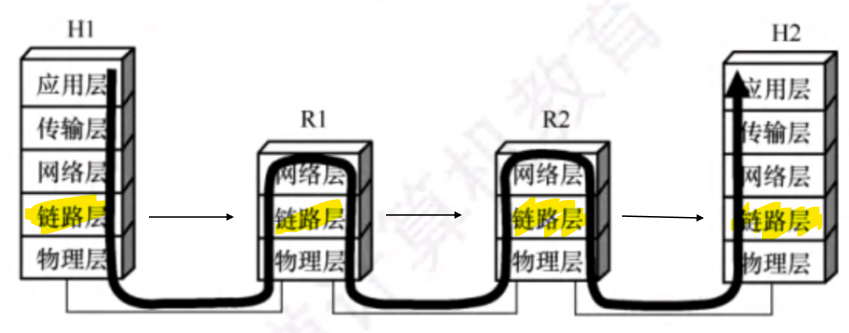
\includegraphics[width=0.7\linewidth]{img/screenshot001}
	\caption{数据流动图}
	\label{fig:screenshot001}
\end{figure}

\textbf{点对点信道相关概念}
\begin{itemize}
	\item[$\rightarrow$] 某些概念对广播信号也是适用的。
	\item \emph{链路}:一个节点到相邻节点的一段物理线路,通常是通信路径的一部分。
	\item \emph{数据链路}:链路+通信协议=数据链路。\\所以也称链路为“物理链路”,数据链
	路为“逻辑链路”。
	\item \emph{帧}:数据链路层对等实体之间进行逻辑通信的协议数据单元。\\数据链路层把
	网络层的数据封装成帧并发送,收到帧后提取数据并上交到网络层。
\end{itemize}

\textbf{为网络层提供服务}:数据链路层为网络层提供三种服务如下。
\begin{itemize}
	\item \emph{无确认的无连接服务}:
	\begin{itemize}
		\item 不需要先建立链路连接和返回确认。
		\item 数据传输的可靠性由高层负责。
		\item 适用于如以太网之类误码率低的信道。
	\end{itemize}
	\item \emph{有确认的无连接服务}:
	\begin{itemize}
		\item 不需要先建立链路连接。
		\item 目的主机收到帧之后需要返回确认。源主机在规定时间内未收到则超时重传。
		\item 适用于如无线通信之类误码率较高的信道。
	\end{itemize}
	\item \emph{有确认的面向连接服务}:
	\begin{itemize}
		\item 帧传输过程分为三个阶段:建立链路$\rightarrow$传输帧 $\rightarrow$释放
		链路。
		\item 目的主机收到帧后需要返回确认。
		\item 适用于可靠性要求较高的场合。
		\item \textbf{链路管理}
		\begin{itemize}
			\item 链路层连接的建立、维持和释放过程称为链路管理。
			\item 首先确认对方是否处于就绪状态,并交换一些必要的信息进行初始化。
		\end{itemize}
	\end{itemize}
\end{itemize}

数据链路层协议有多种,有\textbf{三个基本问题}是共同的:封装成帧、透明传输和差错检验。

\textbf{封装成帧}
\begin{itemize}
	\item 在一段数据的前后分别添加首部和尾部。
	\item \emph{帧长}:数据长度+尾部长度+首部长度。
	\begin{itemize}
		\item 帧的数据长度要尽可能大于首尾部长度,从而使得信息传输效率更高。
		\item 
		帧越长,传输差错的概率越大。
		\item 每种链路层协议都规定了数据部分的长度上限:\emph{最
		大传送单元}。
	\end{itemize}
	\begin{figure}[ht]
		\centering
		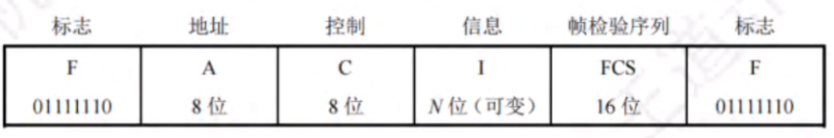
\includegraphics[width=0.7\linewidth]{img/screenshot002}
		\caption{HDLC标准帧格式}
		\label{fig:screenshot002}
	\end{figure}
	\item 
	\emph{帧定界}:首部和尾部中控制信息的一种,确定帧的界限。使得接收方可区
	分出帧的起始和终止(\emph{帧同步})。在HDLC协议中,用标志位F来标志帧的开始和结束。
\end{itemize}

\textbf{透明传输}
\begin{itemize}
	\item 在数据帧中恰好出现了与帧定界符相同的比特组合(F),可能会误以为传输结束。
	\item 用透明传输解决该问题:无论传输什么样的数据都无差错。
\end{itemize}

\textbf{差错检验}
\begin{itemize}
	\item 将错误分为位错和帧错:
	\begin{itemize}
		\item \emph{位错}:某bit出现差错,通常采用\emph{循环冗余检验}(CRC)发现位错
		。
		\item \emph{帧错}:丢失、重复、失序等错误。
	\end{itemize}
\end{itemize}

\textbf{流量控制(非基本问题)}
\begin{itemize}
	\item 限制发送方的发送速率,使其不超过接收方的接受能力。
	\item 在OSI体系架构中,数据链路层具有流量控制能力。
	\item 在TCP/IP体系结构中,流量控制被转移到了传输层。
	\begin{itemize}
		\item 数据链路层:相邻结点流量控制。
		\item 传输层:源到目的端之间的流量控制。
	\end{itemize}
\end{itemize}

\subsection{组帧(封装成帧)}

数据链路层之所以要将数据封装成帧,是为了以帧为单位处理异常(重发等)。
\\组帧主要解决帧定界、帧同步、透明传输等问题。
\\常见的组帧方法通常有四种。

\textbf{字符计数法}
\begin{itemize}
	\item 适用帧首部第一个计数字符来记录该帧字节数。
	\item 多米诺骨牌效应:只要有一帧出错,全盘崩溃。
\end{itemize}

\textbf{字节填充法}
\begin{itemize}
	\item 使用特定字节来定界一帧的开始与结束。
	\begin{figure}[th]
		\centering
		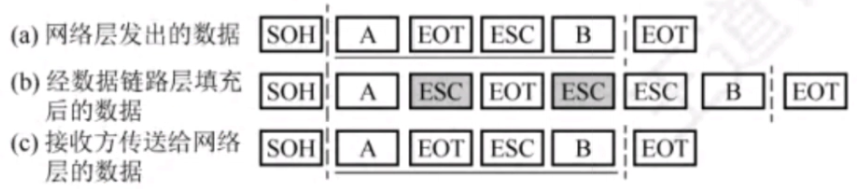
\includegraphics[width=0.7\linewidth]{img/screenshot111}
		\caption{字节填充法}
		\label{fig:screenshot111}
	\end{figure}
	\item 以上图为例:一共有三种特殊字符SOH、EOT、ESC。
	\begin{itemize}
		\item SOE:标识帧开始。
		\item EOT:标识帧结束。
		\item ESC:标识转义。
	\end{itemize}
\end{itemize}

\textbf{零比特填充法}
\begin{itemize}
	\item 使用比特流\lstinline|01111110|标识开始与结束。
	\item 
	发送前:扫描整个数据字段,每遇到5个连续的\lstinline|1|就自动插入\lstinline|0|。
	\item 收到后:每遇到5个连续的\lstinline|1|就自动删除后面紧跟的\lstinline|0|。
	\item 优点:容易用硬件实现,性能优于字符填充法。HDLC协议使用。
	\begin{figure}[th]
		\centering
		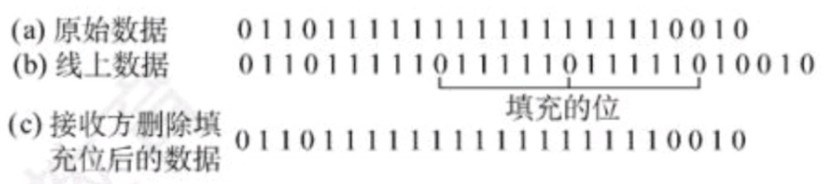
\includegraphics[width=0.7\linewidth]{img/screenshot112}
		\caption{零比特填充法}
		\label{fig:screenshot112}
	\end{figure}
\end{itemize}

\textbf{违规编码法}
\begin{itemize}
	\item 采用违规的物理层变法作为定界符。
	\begin{itemize}
		\item 比如在曼切斯特编码中,合法编码有:“高-低”电平(0)和“低-高”电平(1)。违
		规编
		码有“高-高”和“低-低”。
	\end{itemize}
	\item 优点:违规编码法不需要任何填充技术实现透明传输。局域网IEEE 
	802标准使用。
\end{itemize}

\subsection{差错控制}

\section{网络层}

\subsection{网络层的功能}
\begin{itemize}
	\item OSI曾主张在网络层提供面向连接的虚电路服务。
	\item TCP/IP网络层提供的是无连接的数据服务。
\end{itemize}

\textbf{异构网络互连}

TCP/IP采用标准化协议进行网络互联,参与互联的计算机网络都是用相同的IP协议,可以把互联后
的网络视为一个虚拟IP网络,简称为\emph{IP网络}。

IP网络的好处是:在IP网上主机进行通信,就好像在单个网络上通信看不到各个网络的具体异构细
节。

\begin{figure}[th]
	\centering
	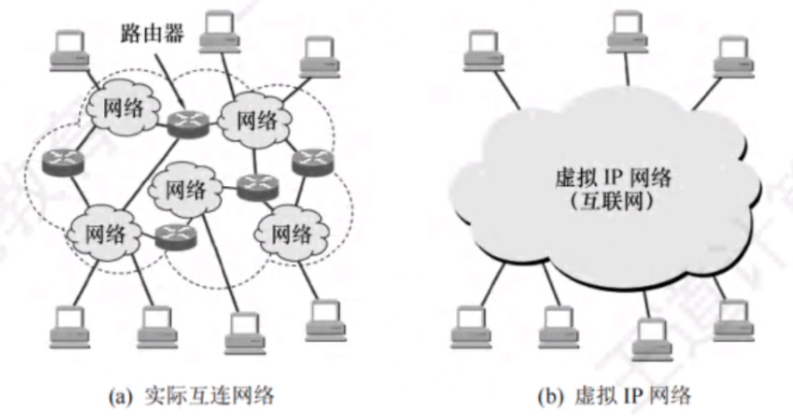
\includegraphics[width=0.7\linewidth]{img/screenadsashot001}
	\caption{IP网络}
	\label{fig:screenadsashot001}
\end{figure}

\begin{smallmdframed}
	各个层次的中继结构:\\
		\emph{物理层}:转发器、集线器;
		\emph{数据链路层}:网桥或交换机;
		\emph{网络层}:路由器;
		\emph{网络层以上}:网关。
\end{smallmdframed}

\textbf{路由与转发}

路由器的两个主要功能:\emph{路由选择}和\emph{分组转发}。
\begin{itemize}
	\item \emph{路由选择}:根据协议构造路由表并定期与相邻路由器交换、更新维护信息,以
	决定分组到达目的地节点的最优路径。
	\item \emph{分组转发}:根据转发表将分组从合适地端口转发出去。
\end{itemize}

\textbf{网络层服务:虚电路和数据报}
\begin{itemize}
	\item \emph{虚电路}:面向连接
	\item \emph{数据报}:无连接
\end{itemize}

\textbf{SDN及其基本概念}

\textbf{拥塞控制}

\subsection{IPv4}
IPv4定义了数据传送基本单元:IP分组的格式及其处理和差错控制细节。

\textbf{IPv4分组格式}

一个IP数据报由首部和数据部分组成。
首部前一部分长度固定,共20B。后一部分长度可变,用于提供错误检测和安全等机制。

\begin{figure}[th]
	\centering
	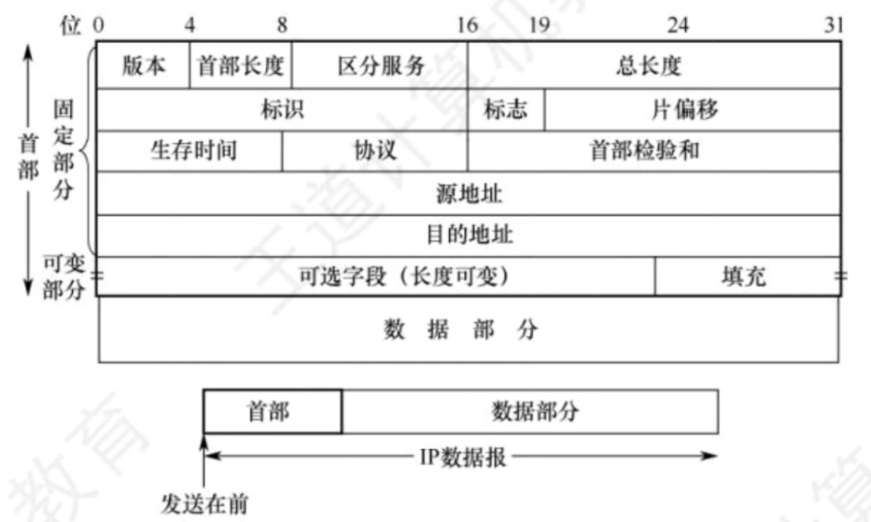
\includegraphics[width=0.7\linewidth]{img/screenadsashot002}
	\caption{IPv4数据报格式}
	\label{fig:screenadsashot002}
\end{figure}

IPv4首部的部分重要字段含义:
\begin{itemize}
	\item 版本号:IP协议的版本,确定如何解释数据包的剩余部分。
	\item 首部长度:由于IPv4数据报首部长度可变,所以需要记录首部长度。
	\item 服务类型(区分服务):将不同类型的IP数据报区分开(如实时与非实时)。
	\item 数据报长度:IP总长度,包括首部长度和数据长度。
	\item 
	生存时间TTL:确保数据报不会永远在网络中循环,每当一台路由器处理数据报时,TTL-1。当$TTL=0$
	则丢弃该数据报。
\end{itemize}

\textbf{IPv4编址}

\subsection{IPv6}

\subsection{路由算法与路由协议}

动态路由算法分为:距离-向量路由算法和链路状态路由算法。

\textbf{距离-向量路由算法}以\textit{Bellman-Ford}算法为基础,不断更新:$$d_x(y)=\min\{c(x,v)+d_v(y)\}$$
其中,$ v $是$ x $的所有邻居。
\\最常见的是RIP算法,用跳数作为距离的度量。

\textbf{链路状态路由算法}向全局节点广播链路信息(只广播与之相邻的节点)。每个节点都是用
链路状态数据独立计算路径。

\subsection{暂存内容:未区分小结}

\textbf{路由器的交换结构}
\begin{itemize}
	\item \emph{经内存交换}:输入端口和输出端口之间的交换是在CPU的直接控制下完成的。当
	一个分组到达输入端口时,会通过中断方式向向路由选择器发出信号。
	\item \emph{经总线交换}:用共享总线将分组直接传送到输出端,不需要处理器干预。输入
	端口分配交换机内部标签,输出端口摘除标签。\\一次只有一个分组能够跨越总线。
	\item \emph{经互联网络交换}:可以并行分发多个不同输出端口的分组。
	\begin{figure}[th]
		\centering
		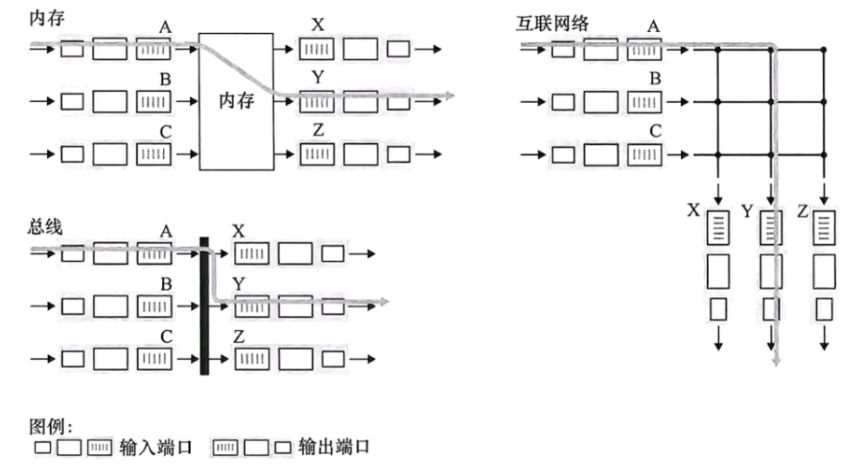
\includegraphics[width=0.7\linewidth]{img/screenadsashot003}
		\caption{三种交换技术}
		\label{fig:screenadsashot003}
	\end{figure}
	
\end{itemize}

\textbf{分组调度}
\begin{itemize}
	\item \emph{先进先出}
	\item \emph{优先权排队}
	\item \emph{循环排队}
	\item \emph{加权公平排队WFQ}:每个类在任何时间间隔内可能收到不同数量的服务。
	\\在类$i$有分组要发送的任何时间间隔中,类$i$将确保收到的服务部分等于$w_i/(\sum 
	w_j)$在最坏的情况下,即使所有类都有分组排队,类$i$也可以分配到带宽的$w_i/(\sum 
	w_j)$。
	\begin{figure}[th]
		\centering
		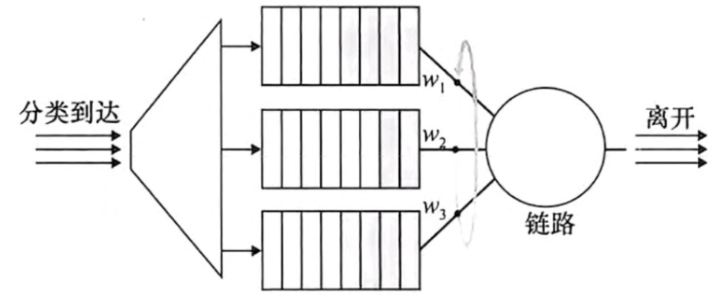
\includegraphics[width=0.7\linewidth]{img/screenadsashot004}
		\caption{加权公平排队}
		\label{fig:screenadsashot004}
	\end{figure}
\end{itemize}

\newpage

\tableofcontents

\appendix
\section{附录1:协议表}

\label{toc}

\end{document}
